% vi:ft=tex
\documentclass[utf8,10pt]{beamer}

\usepackage[english]{babel}
\usepackage{etex}
\usepackage{pgf}
\usepackage[absolute,overlay]{textpos}
\usepackage{tikz}
\usepackage{listings}
\usepackage{graphicx}
\usepackage{pgfplots}
\usepackage{standalone}
\usepackage{enumitem}
%\usepackage[bitstream-charter]{mathdesign}
\usepackage{berasans}
\usepackage[backend=biber,style=alphabetic]{biblatex}
\usepackage{multirow}
\usepackage{mathtools}
\usepackage{ragged2e}
\usepackage{minted}
\usepackage{verbatim}
\usepackage{amssymb}
\usepackage{amsfonts}

\usetikzlibrary{arrows, shapes, positioning, trees,calc,intersections}
\mode<presentation>

% 45 degree rotated column descriptor
\usepackage{adjustbox}
\usepackage{array}

\usetheme[noheader,smallrightmargin,smallleftmargin,nosectionnum,heavyfont]{tud}

\setbeamertemplate{footnote}
{
  %\scriptsize
  \tiny
  \noindent%
  \insertfootnotemark~\insertfootnotetext
}

\setbeamertemplate{enumerate items}[default]
\setbeamertemplate{itemize items}[triangle]

\title[]{Multicore Load Balancing based on behaviour observation}

\author{Philipp Eppelt}

\date{20.11.2015}
\datecity{Dresden}

\einrichtung{Fakultaet Informatik}
\institut{Institut fuer Systemarchitektur}
\professur{Lehrstuhl fuer Betriebssysteme}


\begin{document}

\maketitle

\large

\newcommand{\ft}[1]{\frametitle{\hfill #1}}

% motivation
%%%%%%%%%%%%%%%%%%%%%%%%%%%%%%%%%%%%%%%%%%%%%%%%%%%%%%%%%%%%%%%%%%%%%%%%%%%%%%

\begin{frame}
  \frametitle{fiasco does no balancing \& \\ run-queue balancing disregards
  item size}
  \centering
  \begin{minipage}[l]{.49\columnwidth}
    \includestandalone[width=\columnwidth]{./scheduling_curr_fiasco}
  \end{minipage}
  \begin{minipage}[r]{.49\columnwidth}
    \includestandalone[width=\columnwidth]{./scheduling_curr_rq}
  \end{minipage}
\end{frame}


\begin{frame}
  \frametitle{observe thread's time \& cache usage \\ and balance these}
  \centering
  \begin{minipage}[l]{.49\columnwidth}
    \includestandalone[width=\columnwidth]{./scheduling_curr_bal_time}
  \end{minipage}
  \begin{minipage}[r]{.49\columnwidth}
    \includestandalone[width=\columnwidth]{./scheduling_curr_bal_cache}
  \end{minipage}
\end{frame}


% state of the art
%%%%%%%%%%%%%%%%%%%%%%%%%%%%%%%%%%%%%%%%%%%%%%%%%%%%%%%%%%%%%%%%%%%%%%%%%%%%%%
% SMT


% cache observation
\begin{frame}
  \frametitle{PAM: performance aware meta-scheduler}
\end{frame}
\begin{frame}
  \frametitle{pain metric by Zhuravlev et al. combines ones suffering with the
  hurting of another}
  \centering
  \begin{align*}
    Pain(A|B) &= suffer(A) + hurt(B) \\
    Pain(B|A) &= suffer(B) + hurt(A) \\
    Pain(A,B) &= Pain(A|B) + Pain(B|A)
  \end{align*}
\end{frame}

% communication
\begin{frame}
  \frametitle{deterministic execution times \\ with little variance}

\end{frame}


% service architecture
%%%%%%%%%%%%%%%%%%%%%%%%%%%%%%%%%%%%%%%%%%%%%%%%%%%%%%%%%%%%%%%%%%%%%%%%%%%%%%
\begin{frame}
  \frametitle{haswell cache architecture}
  \centering
  \begin{minipage}[l]{.49\columnwidth}
    \includestandalone[width=\columnwidth]{../haswell_core_layout}
  \end{minipage}
  \begin{minipage}[r]{.49\columnwidth}
    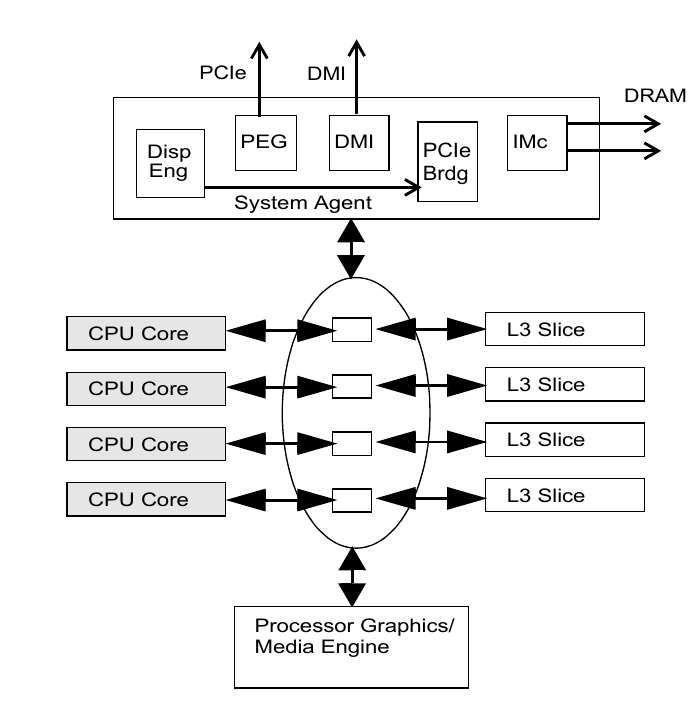
\includegraphics[scale=.27]{../haswell_architecture_by_intel_large_cropped}
  \end{minipage}
\end{frame}

\begin{frame}
  \frametitle{adjustment cycle executed each interval}
  \centering
  \includestandalone[width=.6\columnwidth]{./arch_interval_cycle}
\end{frame}


\begin{frame}
  \frametitle{threads are assigned to the core \\ with the lowest metric value}
  \centering
  \includestandalone[width=.6\columnwidth]{./placementGenerator_inside}
\end{frame}


\begin{frame}
  \frametitle{system layout}
  \centering
  \includestandalone[width=.7\columnwidth]{./threadMapper_layout}
\end{frame}


\begin{frame}[fragile]
  \frametitle{isolation \\of real-time and security critical threads}
  \centering
  \begin{minipage}[c]{\columnwidth}
    \begin{minted}[]{lua}
ld:start({  caps = { },
    scheduler = threadMapperFactory:create(
      L4.Proto.Scheduler,
      "min_prio = 0", "max_prio = 10",
      "rt = false", "sec = true" ),
    log = { "client", "green" }
  },
  "rom/ex_minimal_test");
    \end{minted}
  \end{minipage}
\end{frame}


\begin{frame}
  \centering
  What else can we do with a thread balancer?
\end{frame}


\end{document}
